%%
% This is an Overleaf template for Master's and Bachelor's theses
% using the TUM Corporate Desing https://www.tum.de/cd
%
% For further details on how to use the template, take a look at our
% GitLab repository and browse through our test documents
% https://gitlab.lrz.de/latex4ei/tum-templates.
%
% The tumbook class is based on the KOMA-Script class scrbook.
% If you need further customization please consult the KOMA-Script guide
% https://ctan.org/pkg/koma-script.
% Additional class options are passed down to the base class.
%
% If you encounter any bugs or undesired behaviour, please raise an issue
% in our GitLab repository
% https://gitlab.lrz.de/latex4ei/tum-templates/issues
% and provide a description and minimal working example of your problem.
%%


\documentclass[
  a4paper,	      % paper size (a4paper, a5paper)
  english,	      % define the document language (english, german)
  % BCOR=5mm,           % define a binding offset for the document
  % coverBCOR=1cm,      % define a different binding offset for the cover page
  % coverpage=false,    % disable the cover page (e.g. if a tumcover is used)
  % titlepage=false,    % disable the additional title page
  % oneside,            % use onesided or twosided layout (oneside, twoside)
  % headmarks=true,     % enable headmarks (true, false)
  % font=times          % define main text font (helvet, times, palatino, libertine)
]{tumbook}

% For theses that are printed with a transparent cover it is recommended to
% use the coverpage and provide the proper coverBCOR, so the distance between
% the binding strip and the content is properly set to 1 * logoheight.
% In this case, the publisher and titleback information is most certainly
% empty and the titlepage may be turned off.
%
% For theses that are printed with a soft cover or by a publisher it is
% recommended to create a cover using the tumcover class and therefore turn
% off the coverpage here. In this case, you most certainly have publisher and
% titleback information and you should keep the titlepage option enabled.


% load additional packages
\usepackage{lipsum}
\usepackage{float}
\usepackage{cleveref}
\usepackage{textgreek}

\usepackage[
    backend=biber,
    style=numeric,
]{biblatex}

\addbibresource{thesis.bib}

% thesis metadata
\title{Circular RNAs in estrogen signaling and breast cancer biology}
\subtitle{Zirkuläre RNAs in der Östrogensignalgebung und der Biologie des
Brustkrebses}
\author{Nico Trummer}

\degree{Bachelor of Science (B.Sc.)}
\dateSubmitted{01.04.2021}

\examiner{Prof.\@~Dr.\@ Markus List}
\supervisor{Markus Hoffmann, PhD}


\begin{document}
\setcounter{tocdepth}{4}

\frontmatter
\maketitle
\chapter{Abstract}
\section{Abstract}
The abstract of your thesis goes here.

\lipsum[1-6]

\section{Kurzzusammenfassung}

Deutsche Version des Abstracts.

\lipsum[1-6]
\tableofcontents

\mainmatter
\chapter{Introduction}
\section{Outline}

\begin{itemize}
    \item Describe role of breast cancer in modern health care
    \begin{itemize}
        \item Abundance
        \item Outcomes
    \end{itemize}
    \item Describe current methods for diagnosis and treatment
    \begin{itemize}
        \item Gene panels for risk-assessment of already detected tumors
        \item Shortage of methods for detecting tumors on a molecular basis (need to do more research here)
    \end{itemize}
    \item Describe how circRNAs can improve diagnosis and treatment quality
    \begin{itemize}
        \item Short description of circRNA structure
        \item Increased stability compared to linear RNA biomarkers
        \item Regulatory roles, potential drug targets
        \item Help understanding how well existing treatment methods work (Letrozole, Tamoxifen)
    \end{itemize}
    \item Describe how this thesis approaches the investigation of circRNAs
    \begin{itemize}
        \item Not sure how much detail is necessary here, and how much should be left for materials and methods
    \end{itemize}
\end{itemize}

\section{Introduction}

\lipsum[1-10]

\chapter{Background}
\section{Breast cancer}
Breast cancer is a heterogeneous group of malignancies that primarily
originates in the breast tissue, characterized by the uncontrolled growth of
cells.
It is the most prevalent cancer among women globally, accounting for
approximately 25.2\% of all cancer cases in females and being the second
leading cause of cancer-related deaths among women\supercite{pace_breast_2016}.
The disease can manifest in various forms, with distinct biological behaviors
and responses to treatment.
Notably, breast cancer can be classified based on the presence of hormone
receptors, such as estrogen and progesterone receptors, and the human epidermal
growth factor receptor 2 (HER2)\supercite{eccles_critical_2013}.
The understanding of these subtypes is crucial, as they significantly influence
prognosis and treatment strategies.

\subsection{Types}

Breast cancer is a heterogeneous disease characterized by various subtypes that
differ in their molecular features, clinical behavior, and response to
treatment.
The classification of breast cancer is primarily based on the expression of
hormone receptors (estrogen and progesterone) and the human epidermal growth
factor receptor 2 (HER2).
Understanding these subtypes is crucial for determining prognosis and tailoring
treatment strategies.

One of the most common classifications is based on hormone receptor status,
which divides breast cancer into three main categories: hormone
receptor-positive (HR+), HER2-positive (HER2+), and triple-negative breast
cancer (TNBC).
HR+ breast cancers express either estrogen receptors (ER) or progesterone
receptors (PR) and are typically treated with hormone therapies such as
tamoxifen or aromatase inhibitors\supercite{geyer_molecular_2012}.
Within the HR+ category, there are further distinctions, such as luminal A and
luminal B subtypes.
Luminal A tumors are generally associated with a better prognosis and lower
proliferation rates, while luminal B tumors tend to be more aggressive and may
require chemotherapy in addition to hormone
therapy\supercite{geyer_molecular_2012}.

HER2-positive breast cancer is characterized by overexpression of the HER2
protein, which is associated with aggressive disease and poorer outcomes if
untreated.
However, the advent of targeted therapies, such as trastuzumab, has
significantly improved survival rates for patients with HER2+ breast
cancer\supercite{modi_antitumor_2020}.
Recent studies have also identified a subset of HER2-low breast cancer, which
may not meet the criteria for HER2 positivity but still expresses low levels of
the HER2 protein.
This subtype has been shown to have distinct clinical outcomes and may benefit
from specific therapeutic
approaches\supercite{won_clinical_2022,mutai_prognostic_2021}.

Triple-negative breast cancer (TNBC) is defined by the absence of ER, PR, and
HER2 expression.
This subtype is known for its aggressive nature and limited treatment options,
as it does not respond to hormone therapies or HER2-targeted
therapies\supercite{sizemore_triple_2021}.
TNBC can be further classified into several subtypes based on gene expression
profiles, including basal-like and claudin-low subtypes, which exhibit
different biological behaviors and responses to
treatment\supercite{lehmann_identification_2011}.
The lack of targeted therapies for TNBC has led to ongoing research into novel
treatment strategies, including immunotherapy and combination
therapies\supercite{lehmann_identification_2011}.

In addition to these major classifications, breast cancer can also be
categorized based on histological features, such as invasive ductal carcinoma
(IDC) and invasive lobular carcinoma (ILC).
IDC is the most common type, accounting for approximately 80\% of breast cancer
cases, while ILC is characterized by a distinct growth pattern and may present
unique challenges in diagnosis and
treatment\supercite{mittal_molecular_nodate}.

\subsection{Causes and risk factors}

Breast cancer is a complex disease, with many different causes and risk
factors.
Understanding these factors is key to improving prevention, early detection,
and treatment.
These risk factors can generally be grouped into genetic, lifestyle,
environmental, and — most relevant to this thesis — hormonal influences.

Genetics play a major role in breast cancer risk.
Mutations in genes like BRCA1 and BRCA2 are well-known hereditary factors that
greatly increase the chances of developing breast cancer.
Women with these mutations can face a lifetime risk of up to 80\% for the
disease\supercite{jian_clinical_2017}.
Additionally, having a family history of breast cancer significantly raises the
risk, especially for first-degree relatives of those
affected\supercite{schairer_risk_2013}.

Lifestyle choices also impact breast cancer risk.
Diets high in fat have been linked to a higher risk, possibly because they
affect estrogen levels\supercite{turner_meta-analysis_2011}.
On the other hand, regular exercise and maintaining a healthy weight are
protective factors\supercite{claudia_admoun_etiology_2022}.
Alcohol consumption is another important factor, especially in estrogen
receptor-positive breast cancers\supercite{bao_association_2011}.

Environmental factors, such as exposure to radiation or certain chemicals, can
also raise the risk of breast cancer.
For example, women who received radiation therapy to the chest for other
cancers have a significantly increased risk of developing breast cancer later
in life\supercite{froes_brandao_prolactin_2016}.
Additionally, socioeconomic status plays a role: women from lower-income
backgrounds often have less access to preventive care and early detection
services, which can lead to later diagnoses and worse
outcomes\supercite{cunningham_mind_2013}.

Hormonal influences are critical in breast cancer development.
Factors such as early menarche and late menopause increase risk because of
longer exposure to estrogen\supercite{nounu_sex_2022}.
Reproductive history is another key factor: women who have never given birth or
had their first child later in life are at a higher
risk\supercite{claudia_admoun_etiology_2022}.
Hormone replacement therapy, particularly the combined use of estrogen and
progestin, has also been linked to an increased risk of breast
cancer\supercite{turner_meta-analysis_2011}.

\subsection{Diagnosis}

Diagnosis of breast cancer typically involves a combination of clinical
evaluation, imaging studies, and histopathological examination.
Initial assessments often include mammography, which is a critical screening
tool that can detect tumors before they become
palpable\supercite{hameed_breast_2020}.
In cases where abnormalities are found, further imaging, such as ultrasound or
MRI, may be employed.
Definitive diagnosis is usually achieved through biopsy, where tissue samples
are collected and analyzed microscopically to confirm
malignancy\supercite{hameed_breast_2020}.
The stage at which breast cancer is diagnosed is a critical determinant of
treatment outcomes; early-stage diagnosis is associated with significantly
better prognoses\supercite{getachew_perceived_2020}.
However, barriers to early diagnosis, such as lack of awareness and access to
healthcare facilities, can lead to advanced-stage presentations, which are
linked to poorer clinical
outcomes\supercite{getachew_perceived_2020,dickens_stage_2014}.

\subsection{Treatment}

Treatment options for breast cancer are multifaceted and depend on various
factors, including the cancer subtype, stage, and the patient's overall health.
Standard treatment modalities include surgery, radiation therapy, chemotherapy,
hormone therapy, and targeted therapies.
Surgical options may range from lumpectomy, which conserves breast tissue, to
mastectomy, which involves the removal of one or both
breasts\supercite{metcalfe_contralateral_2014,wu_breast_2014}.
Adjuvant therapies, such as chemotherapy and radiation, are often utilized to
reduce the risk of recurrence, especially in more aggressive forms like
triple-negative breast cancer, which is prevalent among women with BRCA1
mutations\supercite{metcalfe_contralateral_2014}.
Hormonal therapies, such as tamoxifen or aromatase inhibitors, are effective in
hormone receptor-positive breast cancers, while targeted therapies, including
HER2 inhibitors, have revolutionized treatment for HER2-positive
subtypes\supercite{eccles_critical_2013,pace_breast_2016}.
The choice of treatment is increasingly personalized, taking into account
genetic and epigenetic factors that may influence tumor behavior and patient
response to therapy\supercite{khakpour_methylomics_2017}.

\section{Estrogen signaling}

Estrogen signaling plays a pivotal role in the development and progression of
breast cancer, particularly in estrogen receptor-positive (ER+) subtypes.
The primary mechanism of action involves the binding of estrogen to estrogen
receptors (ER\textalpha{} and ER\textbeta{}), which are transcription factors
that regulate gene expression associated with cell proliferation,
differentiation, and survival
\supercite{misawa_estrogen-related_2015,lattouf_lkb1_2016}.
The activation of these receptors can lead to the transcription of genes that
promote tumor growth and metastasis, thereby establishing a direct link between
estrogen signaling and breast cancer pathogenesis
\supercite{feng_cross-talk_2020}.

In ER+ breast cancer, estrogen signaling is often enhanced through various
intracellular signaling pathways, including the phosphoinositide 3-kinase
(PI3K)/AKT and mitogen-activated protein kinase (MAPK) pathways.
These pathways can be activated by growth factors such as HER2, which is
frequently overexpressed in aggressive breast
cancers\supercite{bratton_regulation_2010,salmeron-hernandez_bcas2_2019}.
The crosstalk between estrogen signaling and these pathways not only amplifies
the proliferative effects of estrogen but also contributes to the survival of
cancer cells under therapeutic stress, such as
chemotherapy\supercite{bratton_regulation_2010,george_hypoxia_2012}.
For instance, the interaction between ER\textalpha{} and the PI3K/AKT pathway
has been shown to suppress apoptosis and promote cell survival, which is
critical for tumor
progression\supercite{bratton_regulation_2010,george_hypoxia_2012}.

Moreover, the role of alternative estrogen receptors, such as
ER-\textalpha{}36, has emerged as a significant factor in breast cancer
biology.
ER-\textalpha{}36 is a variant of the classical ER\textalpha{} that mediates
rapid, non-genomic signaling responses to estrogen, influencing cell
proliferation and survival in both ER+ and ER-negative breast cancer
cells\supercite{deng_er-36-mediated_2014,zhang_positive_2011}.
This receptor's activation can lead to enhanced sensitivity to estrogen, even
in cells that typically do not express classical estrogen receptors, thus
complicating treatment strategies\supercite{zhang_positive_2011}.

The influence of estrogen on breast cancer is further complicated by the
presence of co-regulators and other signaling molecules.
For example, the protein CAND1 has been implicated in the regulation of
estrogen signaling pathways, suggesting that it may play a role in metastasis
in ER+ breast cancer\supercite{alhammad_bioinformatics_2022}.
Additionally, the interaction of estrogen with various growth factor signaling
pathways can lead to the upregulation of genes associated with cancer stem cell
properties, thereby promoting tumor heterogeneity and resistance to
therapies\supercite{fillmore_estrogen_2010,xue_sox9fxyd3src_2019}.

\section{Gene Expression}
Gene expression is a complex process consisting of multiple steps that culminate
in the production of functional proteins. This process is tightly regulated at
various levels to ensure the accurate and timely expression of genes in response
to internal and external signals. Here, we provide an overview of the key steps
involved in gene expression, focusing on the transcription and processing of
pre-mRNA into mature mRNA.

\subsection{Transcription and Pre-mRNA Formation} Gene expression begins with
transcription, where RNA polymerase II synthesizes a primary transcript of RNA
from the DNA template. This primary transcript, known as pre-mRNA, contains both
exons (coding sequences) and introns (non-coding
sequences)\supercite{lee_mechanisms_2015}. The pre-mRNA undergoes several
modifications before it can be translated into a protein.

\subsection{Capping and Polyadenylation}
One of the first modifications to occur during pre-mRNA processing is the
addition of a 5' cap, which consists of a modified guanine nucleotide. This cap
is crucial for mRNA stability, nuclear export, and initiation of
translation\supercite{topisirovic_cap_2011}. Following transcription, the
pre-mRNA is also polyadenylated at its 3' end, where a stretch of adenine
nucleotides is added. This poly(A) tail enhances mRNA stability and facilitates
its export from the nucleus to the cytoplasm\supercite{passmore_roles_2022}.

\subsection{Splicing}
The splicing of pre-mRNA is a critical step that involves the removal of introns
and the joining of exons to form a continuous coding sequence. This process is
catalyzed by the spliceosome, a large and dynamic ribonucleoprotein complex
composed of small nuclear RNAs (snRNAs) and numerous protein
factors\supercite{lee_mechanisms_2015}. The spliceosome recognizes specific
sequences at the exon-intron boundaries, facilitating the precise excision of
introns and ligation of exons\supercite{wang_splicing_2008}.

\subsubsection{Alternative Splicing}
A significant aspect of pre-mRNA processing is alternative splicing, which
allows a single gene to produce multiple mRNA isoforms by including or excluding
specific exons. This process is regulated by various splicing factors that
interact with cis-acting elements in the
pre-mRNA\supercite{le_alternative_2015,murphy_therapeutic_2022}. Approximately
95\% of human genes with multiple exons undergo alternative splicing,
contributing to the diversity of the proteome and enabling cells to adapt to
different physiological conditions\supercite{le_alternative_2015}. The
regulation of alternative splicing is influenced by the abundance and activity
of splicing factors, which can change in response to cellular
signals\supercite{wang_mechanism_2015}.

\subsection{Nuclear Export}
Once splicing is complete, the mature mRNA, now devoid of introns and containing
a 5' cap and a poly(A) tail, is exported from the nucleus to the cytoplasm. This
export is facilitated by the nuclear cap-binding complex and other RNA-binding
proteins that ensure the mRNA is properly processed and ready for
translation\supercite{soucek_evolutionarily_2016}. The exon junction complex
(EJC), deposited during splicing, also plays a role in mRNA transport and
stability, further ensuring that only correctly processed mRNAs are
translated\supercite{hir_exon_2016}.

\section{Circular RNAs (circRNAs)}

CircRNAs represent a novel class of non-coding RNAs that have garnered
significant attention in recent years due to their unique structural properties
and diverse biological functions.
Unlike linear RNAs, circRNAs are characterized by a covalently closed loop
structure, which confers increased stability and resistance to degradation by
exonucleases, making them reliable biomarkers and potential therapeutic targets
in various
diseases\supercite{ma_circular_2020,hoque_exploring_2023,wilusz_circular_2017}.
Initially considered mere byproducts of mRNA splicing, circRNAs have now been
recognized for their regulatory roles in gene expression, cellular processes,
and disease mechanisms\supercite{cherubini_foxp1_2019,wilusz_360_2018}.

\subsection{Biogenesis}
During standard gene expression, pre-mRNA is transcribed from DNA.
Splicing then removes introns and joins exons to produce mature
mRNA\supercite{black_mechanisms_2003}.
In conventional splicing, an upstream 5' splice site (donor) connects to a
downstream 3' splice site (acceptor), forming linear mRNA
(\cref{fig:circRNA_splicing}a).
Conversely, for circRNAs, a downstream 5' splice site connects to an upstream
3' splice site in reverse order across at least one
exon\supercite{chen_expanding_2020}.
This backsplicing process is - just like conventional splicing - catalyzed by
the canonical spliceosome\supercite{starke_exon_2015} and results in a circular
RNA molecule (\cref{fig:circRNA_splicing}b).

\subsubsection{Models}

Circular RNAs (circRNAs) are generated through two primary models of
biogenesis: the direct backsplicing model and the lariat-intermediate model.
The direct backsplicing model involves the covalent joining of a downstream 5'
splice site to an upstream 3' splice site, resulting in a circular structure
devoid of a poly(A) tail and 5' cap, which distinguishes circRNAs from linear
RNAs\supercite{zhang_complementary_2014,ferreira_circular_2018}.
This model emphasizes the role of complementary sequences in the introns
flanking the exons, which facilitate the proximity of splice sites necessary
for backsplicing\supercite{zhang_complementary_2014,meganck_engineering_2021}.

In contrast, the lariat-intermediate model posits that circRNAs can also arise
from lariat structures formed during canonical splicing.
In this scenario, introns are excised as lariats, and the remaining exons can
circularize, leading to circRNA
formation\supercite{humphreys_ularcirc_2019,barrett_circular_2015}.
This model highlights the potential for exon skipping, where certain exons are
omitted during splicing, further contributing to circRNA
diversity\supercite{sun_microarray_2020,barrett_circular_2015}.
Both models underscore the complexity of circRNA biogenesis and the interplay
of various molecular mechanisms involved in their
formation\supercite{sharma_recent_2021}.

% TODO: Reference {fig:circRNA_splicing}d

\subsubsection{Alternative splicing}
In conventional splicing, introns are removed and exons are joined linearly.
However, in some cases, exons are skipped or introns are retained, leading to
alternative mature mRNA transcripts based on the same pre-mRNA.
This process is known as alternative splicing\supercite{nilsen_expansion_2010}.
Similarly, circRNAs can be subject to alternative splicing.
This can result in the structures shown in \cref{fig:circRNA_splicing}e and
\cref{fig:circRNA_splicing}f.

\begin{figure}[ht]
    \centering

    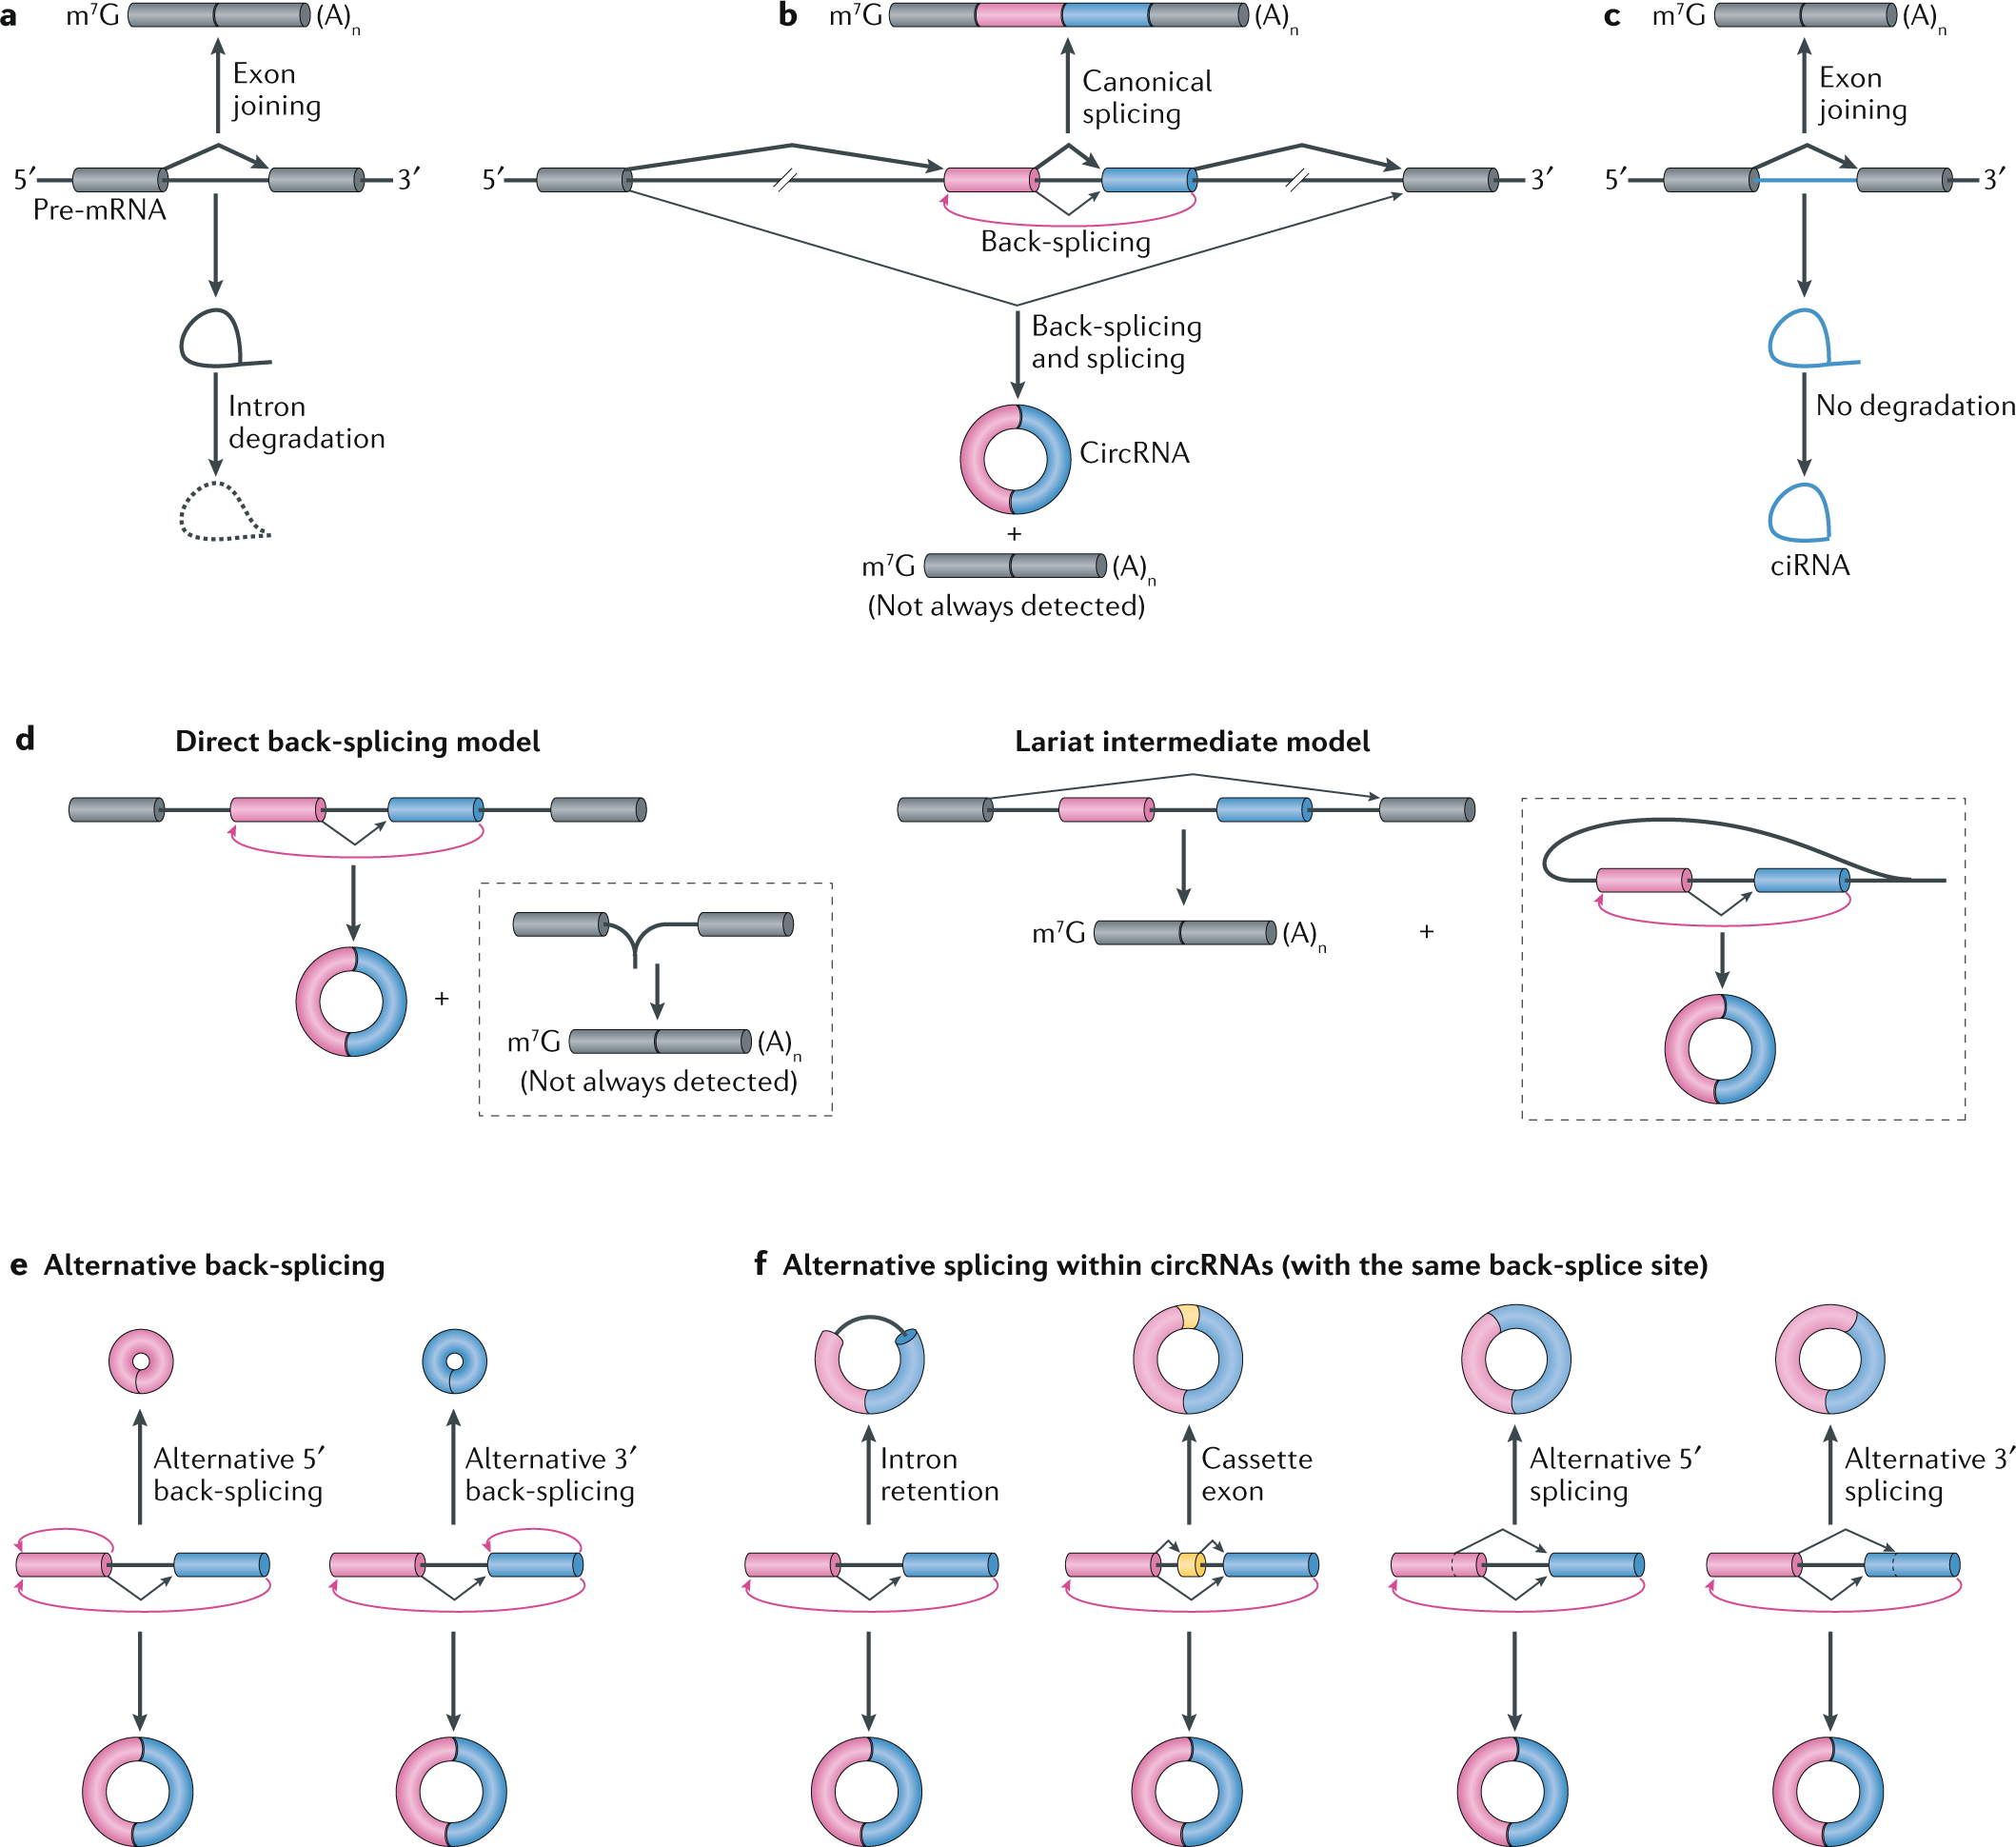
\includegraphics[width=\textwidth]{chapters/background/figures/circRNA-splicing.png}
    \caption{Splicing of circRNAs} % TODO: Add detailed caption
    \label{fig:circRNA_splicing}
\end{figure}

\subsection{circRNA types}
\iffalse
    \subsubsection{Circular intronic RNAs (ciRNAs)}
    Introns typically form a lariat shape during conventional splicing, which is
    generally debranched and degraded soon after splicing
    (\cref{fig:circRNA_splicing}a).
    However, in some cases, introns evade debranching and instead form covalently
    bonded circular RNA molecules (\cref{fig:circRNA_splicing}c), known as circular
    intronic RNAs (ciRNAs) \supercite{chen_expanding_2020,zhang_circular_2013}.

    \subsubsection{Exonic circular RNAs (EcircRNAs)}
    EcircRNAs are generated from exon-skipping events.
    Here, the lariat contains at least one exon and potentially multiple introns.
    The introns are subsequently removed through internal splicing, producing a
    circular RNA molecule composed solely of exonic sequences
    \supercite{xiao_circular_2022, li_biogenesis_2018}.

    \subsubsection{Exon-intron circular RNAs (EIcircRNAs)}
    The formation of EIcircRNAs is similar to that of EcircRNAs, with the exception
    that introns are not completely removed during splicing, resulting in a
    circular RNA molecule containing both exonic and intronic sequences
    \supercite{xiao_circular_2022}.
\fi

\paragraph{Exonic circular RNAs (ecircRNAs)} are the most prevalent type of
circRNAs, primarily formed from back-splicing of exons from protein-coding
genes.
They are typically located in the cytoplasm and can function as sponges for
microRNAs (miRNAs), thereby modulating gene expression and influencing various
cellular processes, including tumorigenesis and cellular differentiation
(Bachmayr-Heyda et al., 2015; Wang et al., 2021).
EcircRNAs have been shown to interact with RNA-binding proteins, which can
further regulate their stability and function (Zang et al., 2018).
Their abundance and stability make them potential biomarkers for various
diseases, including cancers (Li et al., 2021; Wang et al., 2021).

\paragraph{Intronic circular RNAs (ciRNAs)}, on the other hand, are derived
from introns
and are predominantly localized in the nucleus.
They play a role in regulating the transcription of their parental genes and
are characterized by their constrained expression patterns (Ma et al., 2020;
Xie et al., 2023).
ciRNAs are
believed to interact with components of the transcription machinery, thereby
influencing gene expression at the transcriptional level (Reddy et al., 2017).
The nuclear localization of ciRNAs suggests they may have distinct regulatory
functions compared to their ecircRNA counterparts.

\paragraph{Exon-Intron Circular RNAs (EIciRNAs)} are a hybrid form that
includes both
exonic and intronic sequences.
Like ciRNAs, EIciRNAs are also found in the nucleus and have been implicated in
the regulation of gene transcription.
They can enhance the expression of their parent genes by interacting with RNA
polymerase II and other transcription factors (Chen et al., 2022; Su, 2024).
This dual composition allows EIciRNAs to potentially serve as intermediaries in
the regulation of gene expression, bridging the functions of both ecircRNAs and
ciRNAs.

\paragraph{Intergenic circular RNAs (IcircRNAs)} are formed from regions of the
genome
that do not code for proteins and are often less characterized than the other
types.
Their functions remain largely unknown, but they are thought to contribute to
the regulatory networks within cells, possibly by interacting with other RNA
molecules or proteins (Li et al., 2021).
The study of IcircRNAs is still in its infancy, and further research is needed
to elucidate their roles in cellular processes.

\subsection{Biological functions}
circRNAs have emerged as key players in various biological processes,
showcasing
a wide range of functions that contribute substantially to cellular regulation.

\subsubsection{Micro RNA sponging}
One of the most well-documented functions of circRNAs is their ability to act
as miRNA sponges.
This mechanism involves the binding of circRNAs to specific miRNAs, thereby
preventing these miRNAs from interacting with their target mRNAs.
For instance, the circRNA CDR1as has been shown to contain over 60 binding
sites for miR-7, effectively sequestering it and allowing the expression of
miR-7 target genes to
increase\supercite{guo_expanded_2014,yuan_regulatory_2020}.
This competitive endogenous RNA (ceRNA) activity is crucial in regulating gene
expression and has been implicated in various cancers, including gliomas and
gynecological cancers\supercite{dong_expression_2020,song_circular_2016}.
Additionally, circRNAs such as circ-0000437 have been identified as sponges for
miRNAs involved in tumor progression, highlighting their potential as
therapeutic targets\supercite{li_peptide_2021,cui_circular_2022}.

\subsubsection{Protein interactions}
Beyond miRNA sponging, circRNAs also participate in protein interactions.
They can serve as scaffolds for RNA-binding proteins (RBPs), influencing
various cellular processes, including transcription and
splicing\supercite{li_comprehensive_2017,qu_emerging_2017}.
For example, circRNAs can recruit RBPs to specific genomic loci, thereby
modulating the transcriptional landscape of the
cell\supercite{li_comprehensive_2017}.
This interaction can lead to the regulation of gene expression at multiple
levels, further emphasizing the multifaceted roles of circRNAs in cellular
biology\supercite{zhang_important_2024,he_targeting_2021}.
Moreover, some circRNAs have been shown to interact with proteins that are
involved in signaling pathways, such as the Wnt/\textbeta{}-catenin pathway,
thereby influencing cellular proliferation and
differentiation\supercite{peng_novel_2021}.

\subsubsection{Translation into peptides}
In the canonical initiation of translation, ribosomes bind to the 5' cap of an
mRNA \supercite{hinnebusch_mechanism_2012}.
Because circRNAs are circular and lack a 5' cap, they were long thought to be
non-coding \supercite{bao_regulatory_2019,greene_circular_2017}.
However, research has shown that circRNAs with internal ribosome entry sites
can indeed be translated into proteins \supercite{chen_expanding_2020}:

\paragraph{Internal ribosome entry sites (IRES)} In 1988, researchers
discovered that certain viral and cellular mRNAs contain sequences allowing
ribosomes to initiate translation without a 5' cap
\supercite{pelletier_internal_1988, jang_segment_1988}.
These sequences are known as internal ribosome entry sites (IRES).
In 1995, Chen and Sarnow demonstrated that artificially engineered circRNAs
containing an IRES sequence are translated into peptides
\supercite{chen_initiation_1995}.
Later, it was found that some circRNAs naturally possess IRES sequences and can
thus be translated into peptides
\supercite{chen_expanding_2020,legnini_circ-znf609_2017,pamudurti_translation_2017}.
A concrete example for an IRES is the consensus motif for
N\textsuperscript{6}-methyladenosine modification
\supercite{yang_extensive_2017}.

\paragraph{N\textsuperscript{6}-methyladenosine (m\textsuperscript{6}
    A)}  m\textsuperscript{6}A is the most abundant base modification in eukaryotic
RNA \supercite{yang_extensive_2017,li_pivotal_2014,wei_methylated_1975}.
% General introduction to m6A
Research has shown that m\textsuperscript{6}A modification can affect
localization, splicing, translation and degradation of RNA molecules
\supercite{yue_rna_2015,meyer_dynamic_2014}.
The effect of m\textsuperscript{6}A modification on translation is particularly
interesting, as it has been shown that m\textsuperscript{6}A modifications in
3' UTRs can enhance translation
efficiency\supercite{wang_n6-methyladenosine_2015}, while m\textsuperscript{6}A
modifications in 5' UTRs can promote cap-independent translation, especially in
heat shock stress\supercite{zhou_dynamic_2015,meyer_5_2015}.

% Build bridge to IRES-dependent mechanism
m\textsuperscript{6}
A modifications mostly occur in the consensus motif RRm\textsuperscript{6}ACH
(R = purine, H = non-guanine base)
\supercite{csepany_sequence_1990,harper_sequence_1990}, which has been found to
be enriched in circRNAs \supercite{yang_extensive_2017}.
In circRNAs, a single m\textsuperscript{6}A modification is often enough to
initiate translation\supercite{yang_extensive_2017}.

\subsection{Potential applications}
The unique properties of circRNAs, such as their stability, abundance, and
specific expression patterns, make them attractive candidates for various
applications in the field of molecular biology and medicine.
Their potential uses include serving as biomarkers for disease diagnosis and
prognosis, therapeutic targets for drug development, and tools for gene
regulation and editing.

\subsubsection{Biomarkers}
One of the most compelling applications of circRNAs lies in their potential as
biomarkers for cancer diagnosis and prognosis.
Studies have demonstrated that circRNAs can serve as reliable indicators of
tumor progression and treatment response.
For instance, circRNAs exhibit higher expression levels in certain cancers
compared to their linear counterparts, suggesting their utility in liquid
biopsies for non-invasive cancer
monitoring\supercite{bao_prognostic_2020,ren_construction_2017}.
Their stability in bodily fluids such as plasma and saliva further enhances
their applicability as biomarkers, as they are less prone to degradation than
traditional RNA markers\supercite{bao_prognostic_2020,zhang_circular_2018}.
Specific circRNAs, such as hsa\_circ\_0000190, have been correlated with
advanced stages of lung cancer, indicating their potential role in clinical
settings\supercite{luo_plasma_2020}.
Moreover, circRNAs have been implicated in chemoresistance, providing insights
into treatment efficacy and patient
management\supercite{geng_function_2018,feng_functions_2019}.

Beyond their role in cancer, circRNAs are also being explored in the context of
autoimmune diseases and neurological disorders.
For example, circRNAs have been identified as novel biomarkers for rheumatoid
arthritis and multiple sclerosis, highlighting their versatility in reflecting
disease states beyond
oncology\supercite{ouyang_identification_2021,he_exosomal_2019}.
Their expression profiles in various tissues suggest that circRNAs may play a
role in the pathophysiology of these conditions, potentially guiding
therapeutic strategies\supercite{mohammed_circular_2023}.

\subsubsection{Therapeutic targets}
In addition to their diagnostic potential, circRNAs are being investigated as
therapeutic targets.
Their ability to modulate gene expression and interact with microRNAs positions
them as key regulators in cellular processes, including those involved in
cancer stem cell dynamics and immune responses\supercite{cheng_emerging_2023}.
Emerging research indicates that circRNAs can be engineered for therapeutic
purposes, such as enhancing the efficacy of RNA-based therapies like CRISPR and
siRNA\supercite{wesselhoeft_engineering_2018}.
This opens avenues for innovative treatment strategies that leverage the unique
properties of circRNAs to combat diseases more effectively.

\section{Sequencing circRNAs}

Sequencing technologies have revolutionized the field of molecular biology,
enabling researchers to explore the complexities of the genome and transcriptome
with unprecedented depth and accuracy. Traditionally, RNA sequencing (RNA-Seq)
has been performed following poly-A enrichment, a method that selectively
isolates polyadenylated mRNA transcripts. This approach, however, poses
significant challenges for the study of circular RNAs (circRNAs), which lack 5'
caps and poly-A tails, rendering them undetectable in conventional sequencing
protocols\supercite{guo_expanded_2014}. As a result, circRNAs have often been overlooked in
transcriptomic analyses, leading to an incomplete understanding of their
biological roles and regulatory mechanisms.

\subsection{Total RNA sequencing (total-RNA-Seq)}
The advent of total-RNA-Seq has paved the way for a more
comprehensive investigation of circRNAs. Unlike poly-A enrichment methods,
total-RNA-Seq captures all RNA species, including non-coding RNAs such as
circRNAs, thereby providing a more holistic view of the
transcriptome\supercite{panda_identification_2017}. This technique has
facilitated the identification of numerous
circRNAs across various species and tissues, revealing their high abundance and
stability compared to linear RNA
counterparts\supercite{liu_circular_2016,cao_expression_2018}. For instance,
studies have shown that circRNAs can be expressed at levels
significantly higher than their linear isomers, highlighting their potential
functional significance in cellular processes\supercite{liu_circular_2016}.

\section{State of the art}
Circular RNAs (circRNAs) have emerged as significant players in the molecular
landscape of breast cancer, particularly in relation to estrogen signaling and
tumor progression. These non-coding RNAs are generated through back-splicing and
have been implicated in various cellular processes, including the regulation of
gene expression and the modulation of signaling pathways associated with cancer
development\supercite{li_circrna-sfmbt2_2023,tran_new_2020}. The dysregulation
of circRNAs has
been observed in breast cancer, where they can act as competing endogenous RNAs
(ceRNAs), sponging microRNAs (miRNAs) and thereby influencing the expression of
target mRNAs involved in critical pathways such as estrogen receptor (ER)
signaling\supercite{nair_circular_2016,xu_circrna_2022}.

\subsection{CircRNAs in breast cancer}
Recent studies have highlighted specific circRNAs that are associated with
breast cancer subtypes and their clinical implications. For instance,
circRNA-SFMBT2 has been shown to orchestrate ER\textalpha{} activation, contributing to
tamoxifen resistance in breast cancer cells, thereby underscoring the role of
circRNAs in therapeutic resistance\supercite{li_circrna-sfmbt2_2023}. Additionally, circRNAs such as
circTADA2As and circFBXL5 have been identified as regulators of miRNAs that
target key signaling pathways, including the SOCS3 and MAPK/ERK pathways, which
are crucial for cell proliferation and metastasis in breast
cancer\supercite{xu_circtada2as_2019,gao_hsa_circrna_0006528_2019}. This
suggests that circRNAs not only participate in the
pathogenesis of breast cancer but also serve as potential biomarkers for
diagnosis and prognosis\supercite{liu_influence_2021,chen_circepsti1_2018}.

\subsection{CircRNAs and estrogen signaling}
The interaction between circRNAs and estrogen signaling is particularly
noteworthy. Research has demonstrated that ER-positive breast cancer subtypes
exhibit specific circRNA expression profiles that overlap with genes involved in
estrogen signaling pathways\supercite{nair_circular_2016}. For example, circRNA-000911 has
been shown to suppress breast cancer cell proliferation and invasion by sponging
miR-449a, which in turn activates the Notch1 signaling pathway, a known mediator
of estrogen signaling\supercite{wang_comprehensive_2018}. Furthermore, the circRNA-miRNA-mRNA
regulatory networks constructed in various studies have revealed that circRNAs
can modulate the expression of genes related to estrogen response, oxidative
stress, and epigenetic modifications, thereby influencing tumor behavior and
patient outcomes\supercite{xu_circrna_2022,nair_circular_2016}.



\chapter{Materials and Methods}
\section{Data}
This section describes the data used in the study.

\subsection{Mouse models}
Describe the mouse models used in the study and how they were generated.

\subsection{Samples}
Describe the samples used in the study and how they were collected.
Include the timeline plots from the poster.
Explain the different sequencing steps.

\section{Nextflow and nf-core}
\paragraph{Nextflow} is a workflow management system that enables the
development of reproducible and scalable workflows. It allows the creation of
complex pipelines that can be executed on a variety of platforms, from local
machines to cloud computing environments. Nextflow uses a domain-specific
language (DSL) that simplifies the definition of workflows and enables the reuse
of existing components \supercite{di_tommaso_nextflow_2017}. As a result,
Nextflow has become a popular tool in the bioinformatics community.

\begin{figure}[ht]
    \centering
    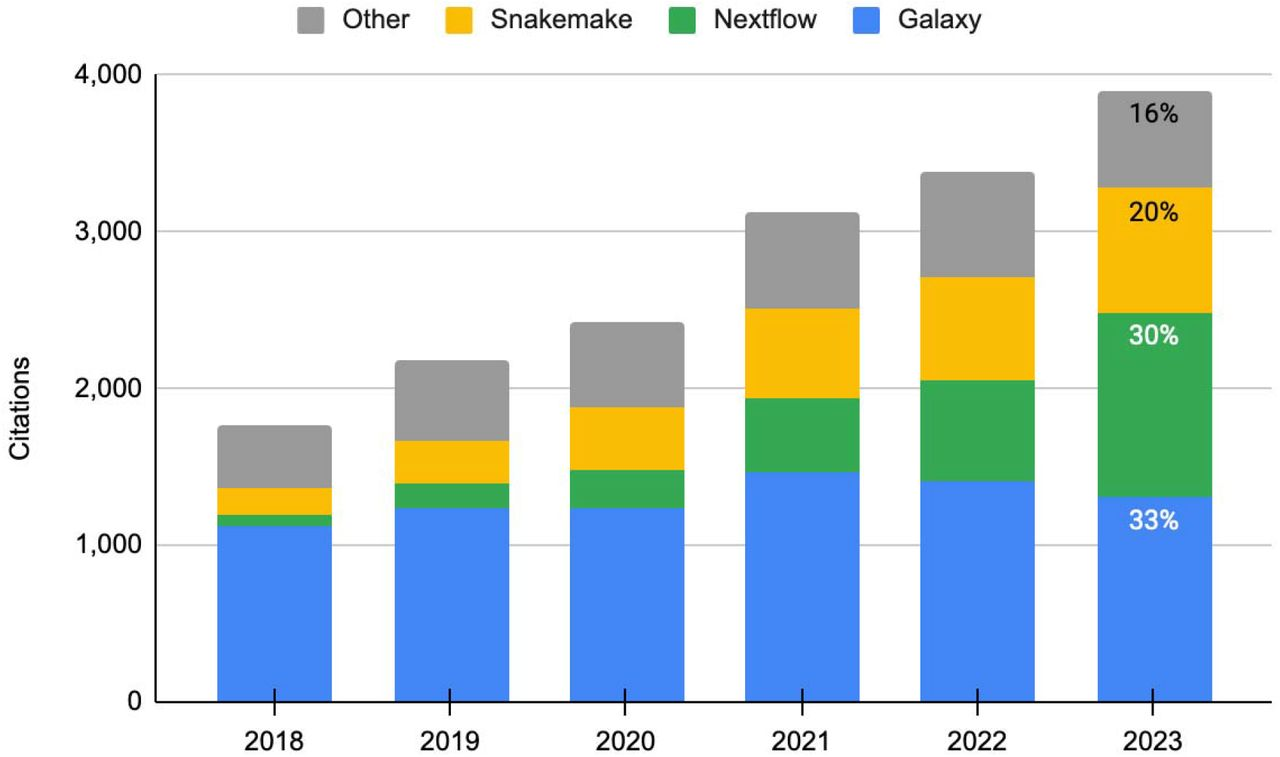
\includegraphics[width=\textwidth]{chapters/materials_and_methods/figures/nextflow_usage.jpg}
    \caption{Workflow management systems} % TODO: Add detailed caption
    \label{fig:nextflow_usage}
\end{figure}

As pointed out by Langer et al. in a recent preprint
\supercite{langer_empowering_2024}, programming-based workflow systems like
Nextflow and Snakemake have gained popularity during the last years, while
GUI-based systems like Galaxy have lost ground. Furthermore, Nextflow has been
the fastest growing workflow system in the last years, with a remarkable 30
percent share of citations in 2023 (\cref{fig:nextflow_usage}). The authors
mostly attribute this to the great quality of the pipelines curated by the
nf-core community \supercite{langer_empowering_2024,grayson_automatic_2023}.

\paragraph{nf-core} is a community-driven project that provides a collection of
high-quality, reproducible, and scalable Nextflow pipelines. These pipelines
cover a wide range of bioinformatics applications, from RNA-seq and ChIP-seq to
single-cell RNA-seq and metagenomics \supercite{ewels_nf-core_2020}. The
community maintains a collection of reusable components, so that developers can
utilize them to speed up the development of new pipelines. The nf-core project
also provides guidelines for best practices in pipeline development, ensuring
that the resulting workflows are robust, efficient, and easy to use
\supercite{ewels_nf-core_2020}.

\section{nf-core/circrna}
The nf-core/circrna pipeline has originally been published by Digby et al. in
2023 \supercite{digby_nf-corecircrna_2023}. Since then, the pipeline has gone
through several updates and improvements. The pipeline can utilize seven
different tools for BSJ detection, including CIRIquant, CIRCexplorer2, circRNA
finder, DCC, find\_circ, MapSplice, and Segemehl. It then annotates the detected
circRNAs using GTF-based and database-based annotation. The pipeline also
extracts the sequences of the circRNAs and quantifies their expression levels
together with the linear transcripts. Finally, the pipeline performs miRNA
interaction analysis using miRanda and TargetScan, and provides several
downstream analyses through a Shiny application. An overview of the pipeline is
shown in \cref{fig:circrna_pipeline}.

\begin{figure}[ht]
    \centering
    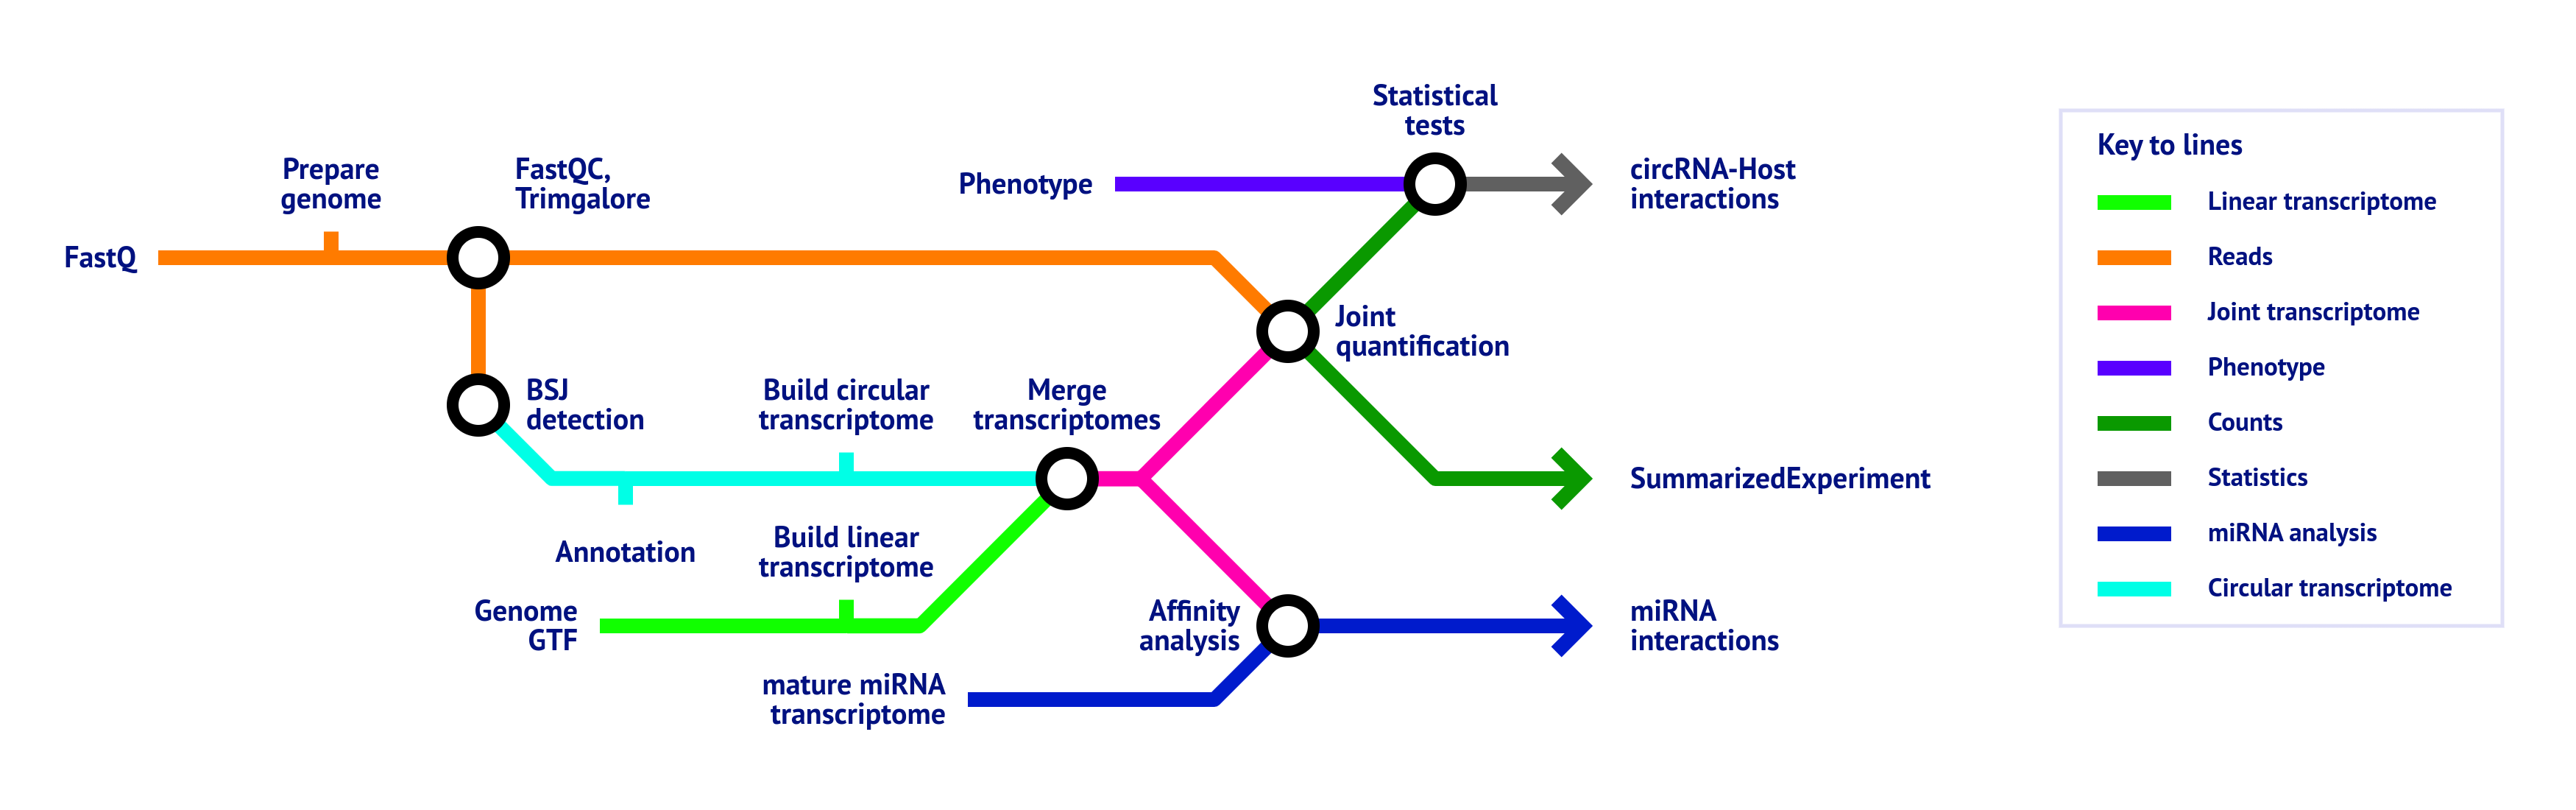
\includegraphics[width=\textwidth]{chapters/materials_and_methods/figures/nf-core_circrna.png}
    \caption{nf-core/circrna} % TODO: Add detailed caption
    \label{fig:circrna_pipeline}
\end{figure}

\subsection{circRNA detection}
What is the main task here?

\subsubsection{CIRIquant}
Describe CIRIquant

\subsubsection{CIRCexplorer2}
Describe CIRCexplorer2

\subsubsection{circRNA finder}
Describe circRNA finder

\subsubsection{DCC}
Describe DCC

\subsubsection{find\_circ}
Describe find circ

\subsubsection{MapSplice}
Describe MapSplice

\subsubsection{Segemehl}
Describe Segemehl

\subsection{circRNA annotation}
What is the main task here?

\subsubsection{GTF based annotation}
Describe GTF based annotation

\subsubsection{Database based annotation}
Describe database based annotation

\subsection{circRNA quantification}

Why is this important?

\subsubsection{psirc-quant}
Describe psirc-quant

\subsection{miRNA interaction analysis}
What can we learn from here?

\subsubsection{miRanda}
Describe miRanda

\subsubsection{TargetScan}
Describe TargetScan

\subsection{Downstream analyses}
\subsubsection{R-shiny}
\subsubsection{Dimensionality reduction}
\subsubsection{Pathway analysis}
\subsubsection{Differential expression analysis}
\subsubsection{Genome browser}


\chapter{Results and Discussion}
\section{circRNAs associated with estrogen signaling}
Results and discussion

\lipsum[1-2]

\section{The role of inferential uncertainty}
Results and discussion

\lipsum[1-2]


\appendix
\chapter{Appendix}
\lipsum[4]

% \backmatter
% \bibliography{}

\printbibliography

\end{document}
